%!TEX root = ../thesis.tex

\chapter{Introduction}\label{ch:introduction}

\section{Problem description}

% something about the Netherlands having used and has been relient on gas for the last ... years, find source

% tell something about the gas numbers from energy trends

% tell why gass is important

% tell that gas is a fosil fuel and thus is not a permanent solution to the energy consumption problem.

% however time and effort has been put into putting steel gas pipes into the ground in the Netherlands

% also in maintaining these pipes.



Steel gas-pipes are placed in the ground where they form corrosion. The amount of formed corrosion is thought to be depending on multiple environment factors. For example, the composition of the soil, the ground water level, and the depth the pipes are placed. In order to prevent the formation of corrosion on the pipes a method called cathodic protection is applied. Cathodic protection uses an electrical system where anodes (metal rods) are placed in the ground near the cathode (the steel pipes). When current is introduced to the system corrosion forms on the anodes and not on the cathode. 

This method is applied on multiple pipe-lines by an energy company called `Cogas' which is located in Almelo. They have collected the environment factors by hand and know how much current is needed per pipe section. Because of the corrosion buildup over time on the anodes and the pipes, at some point in time the amount of current needed exceeds a threshold. At this point it is no longer possible or economically viable to produce the amount of current needed to prevent the corrosion. When this happens more anodes need to be placed or the steel pipes have to be replaced. Cogas wants to be able to predict when this will happen based on their collected data.

The project will be done for ValueA. ValueA provides ICT solutions for utility companies and has Cogas as a client. One of the software solutions ValueA has provided to Cogas is an interactive dashboard where pipe sections with some of their properties are shown. This project will focus on predicting when a pipe section needs maintenance by replacing the pipes or placing more anodes. These predictions could be incorporated in this dashboard.
It is unknown which environment factors (features) leads to the deterioration of the steel pipes. Methods like Supervised Variational Relevance Learning (SUVREL) and Global Metric Learning (GML) could give insight on which features are more important than others in this deterioration process. With the knowledge about the features predictions can be done on the dataset. For this project Learning Vector Quantization (LVQ) will be used to do the predictions. Its performance will be compared to the intuitive and widely used classifier K nearest neighbor (K-nn).

The cathodic protection predictions project is not the only project ValueA is involved with. Another classification problem involves Fraud detection in the energy grid. This problem forms the base of the graduation project of Sebastiaan van Loon. Since both the project of Sebastiaan van Loon and this project will be conducted at ValueA in the same period some collaboration will occur. This collaboration will consist of the development of an abstract module which includes an API that allows the existing software of ValueA to connect to a classifier implementing the abstract module.

This abstract module will be developed to ensure that the ValueA software can connect to a classification module independent of the methods the classification uses. This means that the development of the abstract module does not include the development of the actual classification algorithms and distance measures, which will be developed separately and are not part of the collaboration between Jelle van Wezel and Sebastiaan van Loon.

\section{Goals}

\begin{itemize}
\item Research existing techniques to map LVQ and KNN on a regression problem
\item Research existing methods for feature reduction/relevance
\item Develop a classification module for ValueA which can predict the lifespan of steel gas pipes with LVQ, KNN and a or multiple preprocessing methods like GML and SUVREL.
\item Offer a comparison of the results between the used methods
\item Describe the research, used methods, developed software, and the results.
\end{itemize}

\section{Working Environment}

The student will be partly embedded both in the Intelligent Systems research group within the JBI, and with ValueA at the location of Cogas, a customer of ValueA located in Almelo. It is envisioned that the student will work, on average, two days a week at Cogas and the remaining days at the university and at home. The student will have a meeting at least every fortnight with the first supervisor and will have at least one stand up a week with the third supervisor and/or other employees of ValueA and will attend the monthly meetings of the Intelligent Systems research group. 

The first and second supervisor will provide necessary expertise regarding the classification algorithms and dissimilarity measures used in the project. The third supervisor will provide necessary expertise about both the ValueA software solution and the energy utility market, provide data sets for the training and testing of the classifiers, and evaluate and offer feedback on the software developed.

The student will work on his own laptop and PC, and in case of failure work on a university managed system.  Deployment of software will be done on a cloud environment provided by ValueA. Code revisions will be stored in a GIT repository managed by ValueA. Data which ownership belongs to ValueA will remain in the ValueA cloud environment and will not be copied to the student’s laptops unless explicit permission is granted from ValueA.

\section{Deliverables}

As requested by ValueA the student will develop the software in Python.
\begin{itemize}
\item End of December. Classification module description. A document describing the classification module, its main features and its integration with the existing ValueA software.
\item Start of January. Literature survey. A document summarizing the main findings of a literature review and the relevant references regarding Cathodic protection predictions, LVQ, KNN, Metric learning.
\item End of January. Abstract classification module. An abstract module facilitating the connection of a classifier with the existing software and data of ValueA. (In collaboration with Sebastiaan van Loon.)
\item Mid of February. KNN classification module. A KNN classification module for predictions of gas pipe lifespan.
\item End of March. LVQ classification module. A LVQ module for predictions of gas pipe lifespan with relevance learning as initialization.
\item Mid of April. Test results.
\item Start of May. Thesis draft.
\item Mid of May. Presentation draft.
\item End of May. Presentation to the board of Cogas.
\item End of May. Final presentation, code, and thesis.
\end{itemize}

\section{Cogas}

\begin{figure}[!htb]
\centering
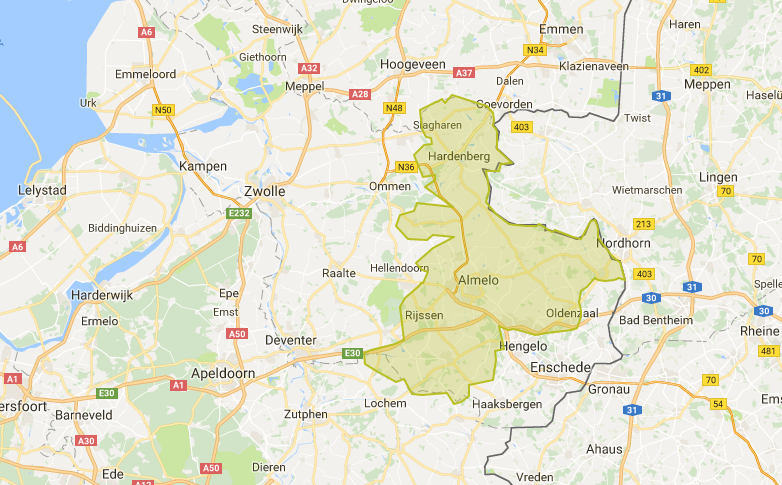
\includegraphics[width=.75\textwidth]{./figures/introduction/cogas_area.png}
\caption{The area Cogas has gas pipelines in.}
\label{fig:intro:cogas-area}
\end{figure}


